During the development of the package has been used an agile methodology, with
similar precepts than the eXtreme programming \cite{eXtreme}, which is based on
simplicity in development, continuous feedback and communication between
team members. This communication has been possible by means of weekly meetings held throughout the year.

For this communication in conjunction with version control \textit{git} has been using,
along with the functionalities available in \textit{Github}. 
Currently, the package is hosted in the repository \href{https://github.com/GAA-UAM/scikit-fda}{https://github.com/GAA-UAM/scikit-fda}.
 This platform offers a
series of tools for the review and control of contributions. There are multiple
workflows designed to carry out version control with \textit{git}, of which we employ
\textit{Gitflow}.


\begin{figure}[Example of git flow branches]{FIG:GITFLOW}{Example of git flow branches \footnotemark}
	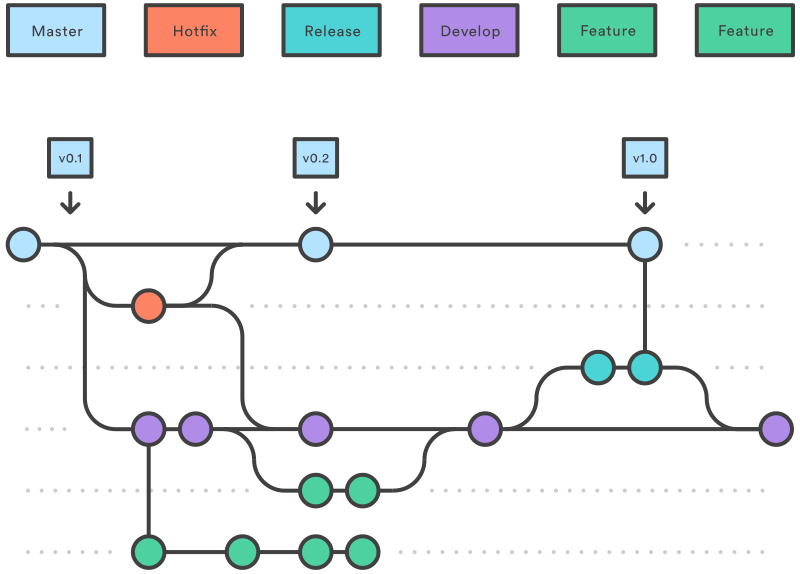
\includegraphics[width=10cm]{gitflow}
\end{figure}

\textit{Gitflow} is a widely used workflow, which uses \textit{git} branches to organize the work.
It structures the code around two main branches: master and develop. The first
is a stable branch, where any built-in commit must be ready to go into
production and generates a new version. The second one, develop, is the code
that will make up the next planned version of the project. To add new code to
these branches, it is necessary to create other auxiliary ones that will be
merged to develop by means of a pull request, after a review process and pass
the bench tests. Figure \ref{FIG:GITFLOW} illustrates the mechanics of this
workflow.




One of the main advantages of using \textit{Github}, over other version control systems,
is the possibility of using a continuous integration mechanism. \textit{Travis CI} has
been used for this purpose, 
which compiles the library and runs the bench tests
each time a commit is made. This has made the development task much easier due to the size of the project, reducing the occurrence of bugs in the code.
In addition, \textit{Travis CI} has made it possible to automate a wide variety of tasks, such as generating the
documentation, compiling or integrating style reviewers.

\footnotetext{Picture from \href{https://es.atlassian.com/git}{https://es.atlassian.com/git}, licensed under a Creative Commons Attribution 2.5 Australia License (accesed on June 2019)}